% !TEX program = xelatex
% DINOv2 arXiv 2304.07193v2 / TMLR 01/2024, Sections 3-7, Appendix A-B.
% Original imagegen draft retained unchanged via graphicx viewports.
% All math, Chinese labels, arrows and grouping redrawn precisely in TikZ.
\documentclass[tikz,border=2mm]{standalone}
\usepackage{fontspec,xeCJK,amsmath,amssymb,graphicx,lmodern}
\setsansfont{Arial}
\setCJKmainfont[Path=/System/Library/Fonts/,BoldFont={STHeiti Medium.ttc}]{STHeiti Light.ttc}
\setCJKsansfont[Path=/System/Library/Fonts/,BoldFont={STHeiti Medium.ttc}]{STHeiti Light.ttc}
\renewcommand{\familydefault}{\sfdefault}
\usetikzlibrary{arrows.meta,calc}
\definecolor{ink}{HTML}{172D40}
\definecolor{muted}{HTML}{536879}
\definecolor{warm}{HTML}{BA632C}
\definecolor{warmbg}{HTML}{FFF8F0}
\definecolor{teal}{HTML}{087E87}
\definecolor{tealbg}{HTML}{F0FAFA}
\definecolor{blue}{HTML}{2E79A6}
\definecolor{bluebg}{HTML}{F0F7FC}
\tikzset{txt/.style={text=ink,font=\fontsize{16}{20}\selectfont,align=center,inner sep=1pt},
 sm/.style={txt,font=\fontsize{13}{17}\selectfont},
 hd/.style={txt,font=\bfseries\fontsize{21}{25}\selectfont},
 ar/.style={-{Stealth[length=2.2mm]},draw=ink,line width=1.2pt,rounded corners=3pt},
 sup/.style={ar,draw=warm,dashed},
 box/.style={rounded corners=5pt,line width=.8pt,draw=teal!55,fill=white}}
\newcommand{\textat}[4]{\node[txt,text width=#3*.3mm]at(#1,#2){#4};}
\newcommand{\smallat}[4]{\node[sm,text width=#3*.3mm]at(#1,#2){#4};}
\newcommand{\headat}[4]{\node[hd,text width=#3*.3mm]at(#1,#2){#4};}
% Original image is 1024 x 1536 pixels, natural PDF size 1024 x 1536 bp.
\newcommand{\art}[7]{\begingroup
 \pgfmathsetmacro{\bt}{1536-#2-#4}\pgfmathsetmacro{\rt}{1024-#1-#3}
 \pgfmathsetlengthmacro{\aw}{#7*.3mm}
 \node[anchor=north west,inner sep=0,outer sep=0]at(#5,#6){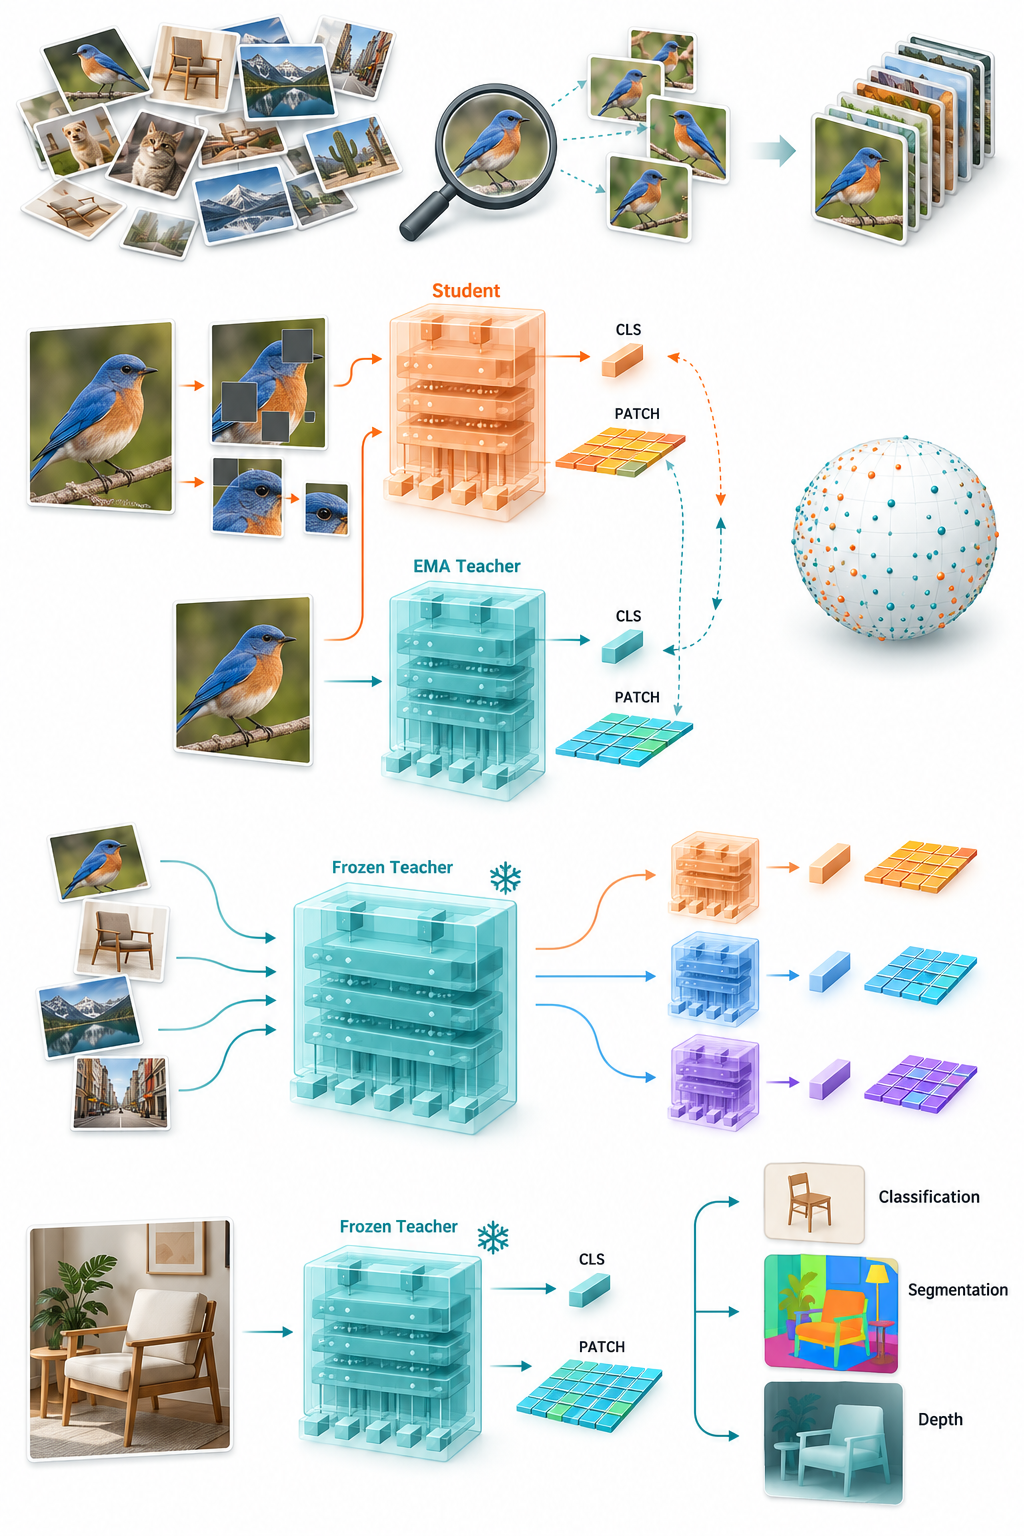
\includegraphics[trim=#1bp \bt bp \rt bp #2bp,clip,width=\aw]{dinov2-imagegen-draft.png}};
\endgroup}
\begin{document}
\begin{tikzpicture}[x=.3mm,y=-.3mm]
\path[use as bounding box](0,0)rectangle(420,1520);
\fill[white](0,0)rectangle(420,1520);
\headat{210}{33}{400}{B\quad 预训练：谁教谁？}
\smallat{210}{76}{398}{教师给目标，学生学预测；两种目标分开算}
\draw[box,fill=warmbg](8,104)rectangle(412,598);
\textat{105}{136}{180}{教师分支}
\textat{315}{136}{180}{学生分支}
\art{175}{598}{139}{169}{54}{170}{102}
\art{207}{314}{125}{140}{256}{170}{102}
\smallat{105}{319}{178}{完整的全局图}
\smallat{315}{319}{178}{遮挡的全局图}
\smallat{315}{351}{178}{也读取局部裁剪}
\draw[ar](105,343)--(105,394);
\draw[ar](315,373)--(315,394);
\art{383}{585}{166}{216}{53}{404}{104}
\art{383}{307}{164}{214}{263}{404}{104}
\textat{105}{568}{180}{EMA 教师}
\textat{315}{568}{180}{可训练学生}

\draw[box,fill=tealbg](8,615)rectangle(412,1017);
\textat{210}{646}{386}{输出分别进入两套独立的头}
\headat{210}{691}{380}{1. DINO：整图目标}
\draw[box](26,725)rectangle(173,790);
\textat{100}{758}{137}{教师 CLS\\目标分布}
\draw[box,draw=warm](247,725)rectangle(394,790);
\textat{321}{758}{137}{学生 CLS\\预测分布}
\draw[sup](178,758)--(241,758);
\smallat{210}{821}{380}{比较不同视图的分布，计算交叉熵}
\headat{210}{868}{380}{2. iBOT：局部目标}
\draw[box](26,901)rectangle(173,966);
\textat{100}{934}{137}{完整图 patch\\目标分布}
\draw[box,draw=warm](247,901)rectangle(394,966);
\textat{321}{934}{137}{遮挡图 patch\\预测分布}
\draw[sup](178,934)--(241,934);
\smallat{210}{994}{384}{只在被遮挡的同一位置比较，不重建 RGB}

\draw[box,fill=warmbg,draw=warm!55](8,1034)rectangle(412,1264);
\headat{210}{1067}{384}{3. 更新参数与目标}
\textat{210}{1110}{384}{损失反传，只用梯度更新学生}
\textat{210}{1157}{388}{$\theta_t\leftarrow m\theta_t+(1-m)\theta_s$}
\smallat{210}{1203}{382}{教师参数取学生的指数滑动平均\\教师目标用 SK（3 轮）；学生用 softmax}

\draw[box,fill=tealbg](8,1281)rectangle(412,1490);
\headat{210}{1314}{385}{4. KoLeo：别挤成一团}
\art{792}{435}{220}{238}{29}{1355}{90}
\textat{270}{1392}{244}{对归一化 CLS 特征\\增大最近邻距离}
\smallat{210}{1463}{384}{作用在首个全局视图的 CLS；不使用类别标签}
\smallat{210}{1512}{400}{虚线箭头：教师监督目标\quad 训练后的大模型再进入蒸馏}
\end{tikzpicture}
\end{document}
